%░▒█▀▀▀█░▒█▀▀▀░▒█▀▀▄░▒█▀▄▀█░░░▒█▀▀▄░▒█▀▀▀░▒█░░▒█░▀█▀░▒█▀▀▀░▒█░░▒█
%░▒█░░▒█░▒█▀▀░░▒█░▒█░▒█▒█▒█░░░▒█▄▄▀░▒█▀▀▀░░▒█▒█░░▒█░░▒█▀▀▀░▒█▒█▒█
%░▒█▄▄▄█░▒█░░░░▒█▄▄█░▒█░░▒█░░░▒█░▒█░▒█▄▄▄░░░▀▄▀░░▄█▄░▒█▄▄▄░▒▀▄▀▄▀
%.:..:..:..:..:..:..:..:..:..:..:..:..:..:..:..:..:..:..:..:.
\section{Orthogonal Frequency Division Multiplexing}

\gls{OFDM} is a modulation technique widely used in high speed wireless communication systems. It divides a channel into a number of equally spaced frequency bands.

%~^~~^~~^~~^~~^~~^~~^~~^~~^~~^~~^~~^~~^~~^~~^~~^~~^~~^~~^~~^~
\subsection{The History of OFDM}
\gls{MCM} was initially used for military \gls{HF} radios in the years 1950--1960. The use of orthogonal frequencies for transmission first appears in a 1966 patent by \emph{Robert W. Chang} of Bell Laboratories\cite{ofdm_intro}.
The proposal to use \gls{FFT} to generate orthogonal signals originally surfaced in 1969. Parallel data streams and \gls{FDM} would be used, but with overlapping sub-channels. The merits of this method include:
\begin{itemize}
	\item Avoiding the use of high speed equalization.
	\item Mitigation of impulsive noise and multi-path distortion.
	\item Maximal utilization of available bandwidth.
\end{itemize}
The earliest adoption of OFDM is seen in military communication.
\begin{figure}[!ht]
	\centering
	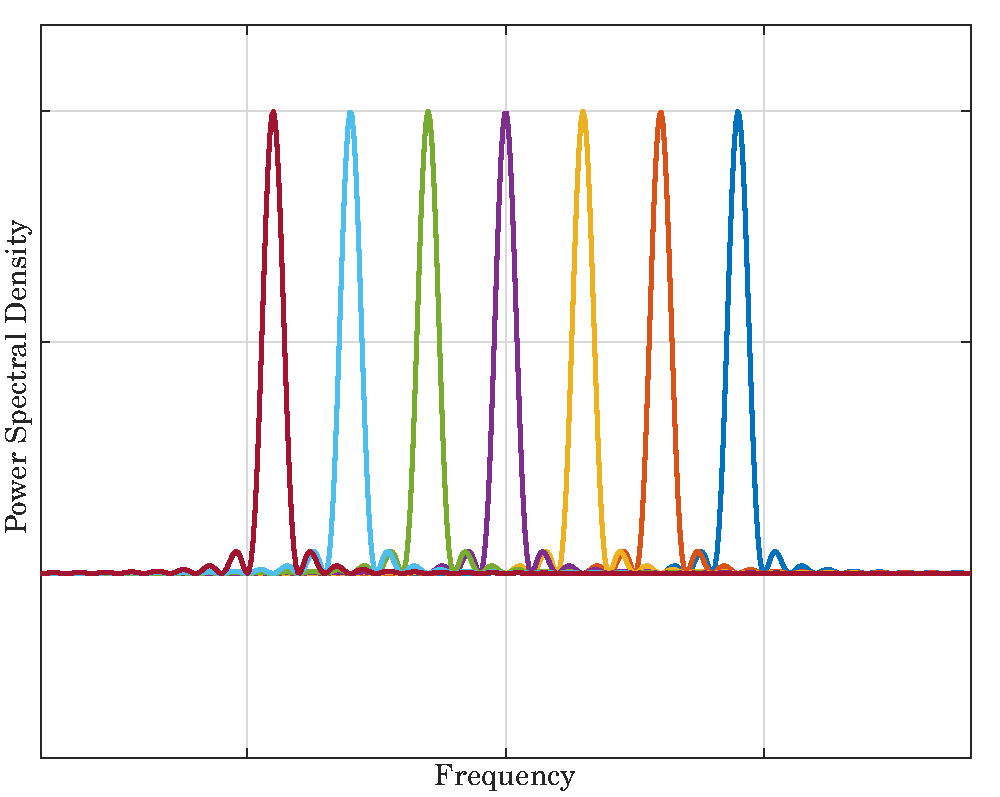
\includegraphics[width=0.8\textwidth]{Graphics/LiteratureReview/fdm.pdf}
	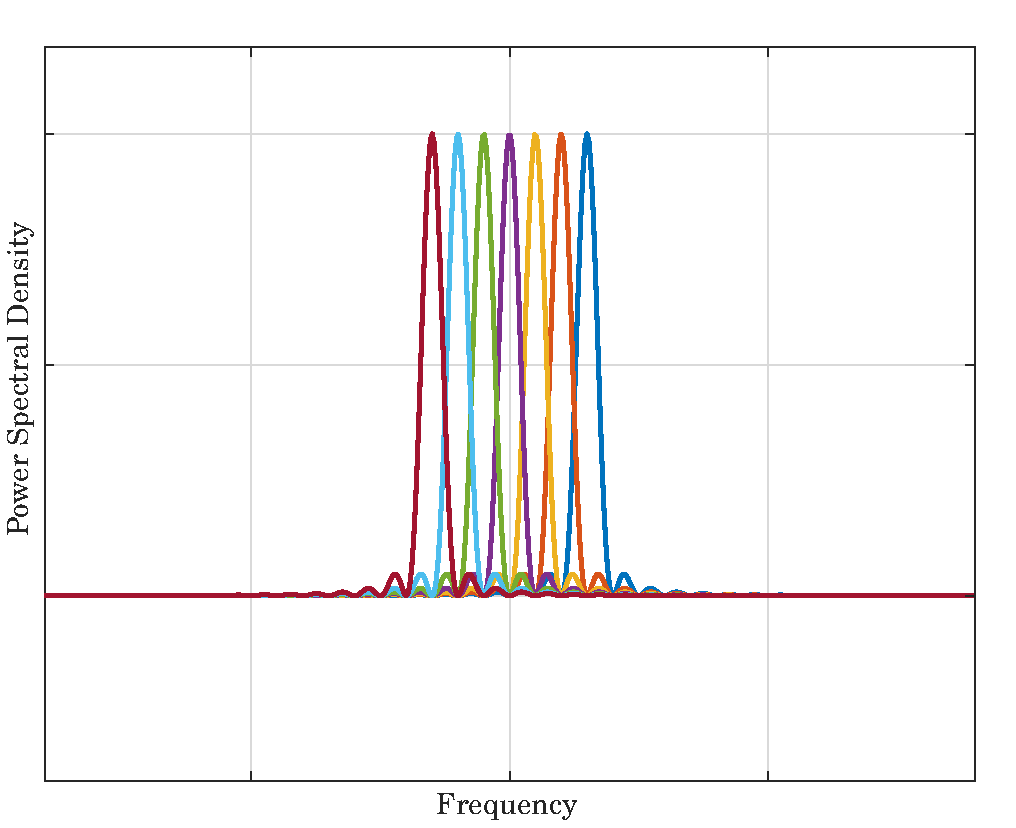
\includegraphics[width=0.8\textwidth]{Graphics/LiteratureReview/ofdmPSD.pdf}
	\caption{Comparison of OFDM and FDM spectral efficiency}
	\label{fig:litRev:fdm}
\end{figure}

Thereafter, some fundamental improvements were incorporated into OFDM, most notably the inclusion of a \emph{cyclic prefix} in the early 1980s. The technique started to be considered for practical adoption in the mid 80s. In 1987, particularly, \emph{Lassalle} and \emph{Alard}, based in France, considered the use of OFDM for radio broadcasting. They noted the necessity of combining \gls{FEC} with \gls{OFDM}.

A novel application of OFDM was pioneered by \emph{Cioffi} and others at \emph{Stanford}, who showed its potential as a modulation technique for \gls{DSL} applications. In 1999, the first OFDM \gls{WLAN} standard \emph{802.11a} was published, followed in succession by \emph{802.11n} and \emph{802.16d}. However, the most widely deployed \gls{WLAN} standard is \emph{802.11b}, which uses \gls{DSSS}. OFDM is the basis of many telecommunication standards.

%,-.,-.,-.,-.,-.,-.,-.,-.,-.,-.,-.,-.,-.,-.,-.,-.,-.,-.,-.,-.
\subsubsection{IEEE 802.11 Standard}
The \emph{IEEE 802.11} specification is a standard that specifies the set requirements for the physical layer and a medium access control layer. The standard provides two definitions for physical layers-- \emph{802.11b} for \SI{2.4}{\giga\hertz} operation and \emph{802.11a} for \SI{5}{\giga\hertz} operation\cite{802.11}.

\emph{802.11a} and \emph{802.11b} are not inter-operable unless the equipment in use has dual band capability. These are the standard's specifications:
\begin{table}
	\centering
	\renewcommand{\arraystretch}{1.5}
	\begin{tabular}{l l}
		\emph{Parameter} & \emph{Value}\\
		\hline
		Modulation technique & BPSK, QPSK, 16-QAM, 64-QAM \\
		Coding rate & 1/2, 2/3, 3/4 \\
		Number of subcarriers & 52 \\
		Number of pilots & 4 \\
		Symbol duration & \SI{4}{\micro\second} \\
		Guard interval & \SI{800}{\nano\second} \\
		Sub-carrier spacing & \SI{312.5}{\kilo\hertz} \\
		\SI{3}{\decibel} bandwidth & \SI{16.56}{\mega\hertz} \\
		Channel spacing & \SI{20}{\hertz}
	\end{tabular}
	\label{tab:litRev:802.11}
\end{table}
All data sub-carriers use the same modulation format within a given burst but this can vary from burst to burst.

%~^~~^~~^~~^~~^~~^~~^~~^~~^~~^~~^~~^~~^~~^~~^~~^~~^~~^~~^~~^~
\subsubsection{OFDM Variants}
Variants of OFDM follow the standard implementation but possess additional attributes. Some of these include:
%`'`'`'`'`'`'`'`'`'`'
\paragraph{Coded OFDM} This is a variant of OFDM in which error correcting code is incorporated into the signal.
%`'`'`'`'`'`'`'`'`'`'
\paragraph{Flash OFDM} This is a fast-hopped version of OFDM which utilized multiple tones and fast hopping to spread signals over a given spectrum band.
%`'`'`'`'`'`'`'`'`'`'
\paragraph{Vector OFDM} This variant uses \gls{MIMO} techniques. It is a proprietary variant being developed by CISCO Systems. \gls{MIMO} techniques involve the use of multiple antennas to transmit and receive such that multi-path effects can be utilized to enhance signal reception and transmission speeds.
%`'`'`'`'`'`'`'`'`'`'
\paragraph{Wideband OFDM} A form of OFDM that uses such a large degree of spacing between its sub-channels that frequency errors between transmitter and receiver do not affect communication performance. It is particularly applicable to Wi-Fi systems.

%~^~~^~~^~~^~~^~~^~~^~~^~~^~~^~~^~~^~~^~~^~~^~~^~~^~~^~~^~~^~
\subsection{Principles of OFDM}
\gls{OFDM} is a type of \gls{MCM}, with the most apparent advantage of being that simultaneous transmission of \(N\) symbols over \(N\) sub-carriers reduces symbol rate \(1/N\) times the original. This also means that symbol duration is increased \(N\) times, which extenuates \gls{ISI}, consequently reducing the need for channel equalization.

Recovering the signals of the sub-channels at the receiver can be achieved through:
\begin{itemize}
	\item Spacing sub-carrier frequencies such that the spectra of \(N\) sub-channels do not overlap. \(N\) \gls{BPF}s are then used to separate these sub-channels, each requiring a sharp frequency response. This is the method used in \gls{OFDM}.
	\item Allowing the sub-carriers which are orthogonally spaced by \(1/T\) to overlap. The signals in the sub-carriers are recovered from the sub-carriers using correlators in the receiver. This method is used in \gls{OFDM}.
\end{itemize}
The advantages of \gls{OFDM} over single carrier modulation are:
\begin{enumerate}
	\item The Nyquist's rate for a given channel can be approached without the use of sharp cutoff filters.
	\item It elongates symbol period, countering the effects of \gls{ISI} due to channel dispersion and multipath interference.
	\item OFDM divides the frequency band into narrow bands, reducing sensitivity to wide-band impulse noise and frequency selective fading. The complex fading coefficient on each sub-band signal can be removed by multiplying the signal with the conjugate of the fading coefficient.
	\item Different modulation formats can be used on different sub-carriers depending on sub-channel noise.
	\item OFDM is digitally implementable using \gls{IDFT}/\gls{DFT} pair through their \gls{IFFT}/\gls{FFT} algorithm pair, greatly reducing system complexity.
\end{enumerate}
Wide adoption of OFDM in recent years has been commensurate with increasing computing power.

%,-.,-.,-.,-.,-.,-.,-.,-.,-.,-.,-.,-.,-.,-.,-.,-.,-.,-.,-.,-.
\subsubsection{OFDM Signal and Spectrum}
The final form of an OFDM signal can be a \emph{baseband} or a \emph{bandpass} signal. It is always baseband for wired systems due to limited bandwidth. In wireless systems, baseband signals are up-converted to the \gls{RF} band for transmission.
%`'`'`'`'`'`'`'`'`'`'
\paragraph{Baseband OFDM Signal} Its general form is expressed as:
\begin{align*}
	s(t) &= \sum_{i=0}^{N-1}s_i(t) = \sum_{i=0}^{N-1}A_i \cos (2\pi f_i t + \phi_i) & 0 \leq t \leq T
\end{align*}
\begin{mathDef}
	\mathSymb{A_i}{Amplitude of \(i\)\nth subcarrier}
	\mathSymb{f_i}{Frequency of \(i\)\nth subcarrier}
	\mathSymb{\phi_i}{Phase of \(i\)\nth subcarrier}
	\mathSymb{N}{Number of subcarriers}
	\mathSymb{T}{Symbol period of the data}
\end{mathDef}
Depending on the modulation format (\gls{ASK} or \gls{PSK}), \(A_i\) or \(\phi_i\) respectively are determined by data while the others remain constant.
%`'`'`'`'`'`'`'`'`'`'
\paragraph{Proof of orthogonality} For the sub-carriers to be orthogonal, \(f_i\) must be integer multiples of \(1/2T\) and the minimum frequency separation between them must be \(1/T\). The subcarrier frequencies are taken to be:
\begin{align}
	f_i &= iR_s = \frac{i}{T} & i = 0, 1, \ldots, N-1
	\label{eq:litRev:subCarriers}
\end{align}
\begin{mathDef}
	\mathSymb{R_s}{Symbol duration}
\end{mathDef}
If we take the lowest subcarrier frequency as \(f_0\), the sub-carrier frequencies are: \(f_0, f_0 + R_s, f_0 + 2R_s, \ldots, f_0 + (N-1)R_s\). In practice, \(f_0\) isn't \SI{0}{\hertz} to avoid a DC offset in the \gls{DAC}.
With the subcarrier frequencies in equation \eqref{eq:litRev:subCarriers}, orthogonality is verified by:
\[
	\int_0^T s_i(t)s_j(t) \cdot dt =
	\begin{cases}
		{A_0}^2 T\cos^2 \phi_0 & i = j = 0 \\
		\frac{1}{2}{A_i}^2 T & i = j \neq 0 \\
		0 & i \neq j
	\end{cases}
\]
This is the proof of orthogonality between subcarriers and it holds for all values of \(A_i\), \(A_j\) and \(\phi_i\), \(\phi_j\) for the frequency allocation of equation \eqref{eq:litRev:subCarriers}\cite{ofdm_intro}.

The frequency spectrum of the \gls{OFDM} signal is characterized by its \gls{PSD}. With the assumption that the data on each subcarrier is independent of others, overall \gls{PSD} is a superposition of the PSDs of all sub-channel signals\cite{fuqin}:
\begin{equation}
	S(f) = \sum_{i=0}^{N-1}S_i(f)
	\label{eq:litRev:generalPSD}
\end{equation}
\begin{mathDef}
	\mathSymb{S(f)}{Overall PSD of the OFDM signal.}
	\mathSymb{S_i(f)}{PSD of the \(i\)\nth sub-channel signal \(s_i(t)\)}
\end{mathDef}
For \(i \neq 0\), where the modulation format is \gls{MASK} or \gls{QAM} with symmetrical constellation, the PSD of the \(i\)\nth sub-channel's signal is:
\begin{align}
	S_i(f) &= \frac{1}{2}{A_{avg}}^2T \left[ \left(\frac{\sin \pi(f-f_i)T}{\pi(f-f_i)T}\right)^2 + \left(\frac{\sin \pi(-f -f_i)T}{\pi(-f-f_i)T}\right)^2\right] & i\neq 0
	\label{eq:litRev:ofdmPSD}
\end{align}
For QAM, \({A_{avg}}^2 = 2{\sigma_a}^2\) whereas it is \({\sigma_a}^2\) for \gls{MASK}.
\begin{mathDef}
	\mathSymb{{\sigma_a}^2}{Amplitude variance of \emph{in-phase} and \emph{quadrature} components.}
\end{mathDef}
For \gls{MPSK} modulation, the PSD function is the same, except that \(A_{avg}\) is equal to the \gls{PSK} amplitude.

When \(i=0\), \(s_i(t) = A_i \cos \phi_i\) is a baseband signal which is equivalent to the in-phase channel data for \gls{QAM} or \gls{PSK}. Its \gls{PSD} is given by:
\begin{equation}
	S_0(f) = {\sigma_a}^2T (\sinc \pi f T)^2 = \frac{1}{2}{A_{avg}}^2T(\sinc \pi f T)^2
	\label{eq:litRev:0thPSD}
\end{equation}
Combining \eqref{eq:litRev:generalPSD}, \eqref{eq:litRev:ofdmPSD} and \eqref{eq:litRev:0thPSD} then normalizing the PSD by its maximum and only showing the positive frequency part:
\begin{align}
	S(f) &= \sum_{i=0}^{N-1} \left( \frac{\sin \pi(f - f_i)T}{\pi(f - f_i)T} \right)^2 & f \geq 0
	\label{eq:litRev:simplePSD}
\end{align}
Each member of PSD has the shape of a squared \(\sinc\) function. The first PSD's null is at \((f-f_i) = 1/T\). As separation between sub-carriers is \(1/T\), this means that the first null point coincides with the peak of the PSDs of immediately adjacent sub-channel signals.

The null bandwidth of the composite \gls{PSD} of an \(N\) sub-carrier baseband OFDM signal is:
\begin{align*}
	B_{null} &= \frac{N}{T} = \frac{N}{R_s} \\
	B_{null-to-null} &= \frac{2N}{T} = 2NR_s
\end{align*}

%`'`'`'`'`'`'`'`'`'`'
\paragraph{Passband OFDM Signal}

When an \gls{RF} bandwidth is allocated to an OFDM signal, subcarrier frequencies are chosen to be symmetrically distributed around a nominal carrier frequency. Thus, the subcarrier frequencies are:
\begin{align*}
	f_i &= f_c - \frac{N-1}{2T} + \frac{i}{T} & i = 0,1,\ldots,N-1
\end{align*}
\begin{mathDef}
	\mathSymb{f_c}{Nominal \gls{RF} carrier frequency.}
\end{mathDef}
This means:
\[
	f_c - \frac{N-1}{2T} \leq f_i \leq fc + \frac{1}{2T}
\]
The passband OFDM signal can be expressed:
\begin{align*}
	s(t) &= \sum_{i=0}^{N-1} A_i \cos \left[ 2\pi \left( f_c - \frac{N-1}{2T} + \frac{i}{T}\right)t + \phi_i \right] & 0 \leq t \leq T
\end{align*}
The sub-channels at \gls{RF} frequencies need not be orthogonal to each other since demodulation is not performed at RF frequencies\cite{fuqin}. The RF-band OFDM signal is first down-converted to baseband frequencies where subcarrier frequencies are multiples of \(1/2T\)\cite{fuqin}. At this point, it's then demodulated.

The passband OFDM signal is a frequency shifted version of the baseband signal. When data on each sub-channel is independent of the others, the total \gls{PSD} is a sum of individual PSDs:
\[
	S(f) = \sum_{i=0}^{N-1} \left( \frac{\sin \left[ \pi(f - {f_c}^\prime - \frac{i}{T})T \right]}{\pi(f - {f_c}^\prime - \frac{i}{T})T} \right)^2
\]
\begin{mathDef}
	\mathSymb{{f_c}^\prime}{Frequency shift of passband OFDM signal}
\end{mathDef}
The frequency shift can be found by mixing the baseband OFDM signal with an \gls{RF} signal of frequency \({f_c}^\prime\) while keeping the \gls{USB} but discarding the \gls{LSB}. The mixing frequency is the nomical carrier frequency with an offset:
\[
	{f_c}^\prime = f_c - \frac{N-1}{2T}
\]
The null-to-null bandwidwth is given by:
\[
	B_{null-to-null} = \frac{N + 1}{R_s}
\]
Transition bands of passband PSDs get sharper and sidelobes get lower as \(N\) increases. Normalized null-to-null bandwidth approaches 1 as \(N\to\infty\)\cite{fuqin}.

The Nyquist rate of a channel with a rectangular frequency response is equal to its passband bandwidth. This is achievable with OFDM since its normalized passband frequency bandwidth is 1\cite{fuqin}.


%~^~~^~~^~~^~~^~~^~~^~~^~~^~~^~~^~~^~~^~~^~~^~~^~~^~~^~~^~~^~
\subsection{OFDM Modulator and Demodulator}
There are two differentiated implementations of the OFDM modem:
\begin{itemize}
	\item \emph{Analog modem.} Modulation by multipliers and demodulation by correlators.
	\item \emph{Digital modem.} Modulator uses \gls{IDFT} and demodulator uses \gls{DFT}.
\end{itemize}

%~^~~^~~^~~^~~^~~^~~^~~^~~^~~^~~^~~^~~^~~^~~^~~^~~^~~^~~^~~^~
\subsubsection{Analog OFDM Modem}
This implementation is a scaled version of single carrier communication system. Therefore, for a large number of sub-carriers, it becomes prohibitively complex and impractical. 
%`'`'`'`'`'`'`'`'`'`'
\paragraph{Transmitter side} The process by which the passband OFDM signal is generated:
\begin{figure}[!h]
	\centering
	\resizebox{\textwidth}{!}{
		\input{Graphics/LiteratureReview/analogMod.pdf_tex}
	}
	\caption{Analog OFDM Modulator}
\end{figure}
\begin{itemize}
	\item Serial data bits \(\{a_k\}\) are converted by the \(1:N\) serial-to-parallel converter into \(N\) data streams.
	\item The bits in each stream are then mapped to a symbol, typically denoted by a complex number.
		\begin{align*}
			d_1 &= A_i \exp (j\phi_i) = I_i + jQ_i & i = 0,1,\ldots, N-1 \\
			I_i &= A_i \cos \phi_i \\
			Q_i &= A_i \sin \phi_i
		\end{align*}
		\begin{mathDef}
			\mathSymb{I_i}{Symbol in-phase component.}
			\mathSymb{Q_i}{Symbol quadrature component.}
		\end{mathDef}
	\item \(d_i\) is modulated onto the \(i\)\nth subcarrier in the modulator. Sub-channels may have different modulation formats. There are \(N\) modulators, each comprising a subcarrier frequency oscillator. The separate sub-channel signals are then added by the adder to generate the baseband OFDM signal.
	\item To get a passband OFDM signal, the baseband signal is fed into an RF mixer which has a reference signal of frequency \({f_c}^\prime\) and a \gls{BPF} which rejects the resulting \gls{LSB} of the mixer output. The passband signal's spectrum is centered at \(f_c\).
\end{itemize}

%`'`'`'`'`'`'`'`'`'`'
\paragraph{Receiver side} The processing in this stage reverses the transmitter's work\cite{ofdm_intro}.
\begin{figure}[!h]
	\centering
	\resizebox{\textwidth}{!}{
		\input{Graphics/LiteratureReview/analogDemod.pdf_tex}
	}
	\caption{Analog OFDM Demodulator}
\end{figure}
\begin{itemize}
	\item The passband signal gets translated to baseband through a down-converter with a reference frequency \({f_c}^\prime\).
	\item The \gls{USB} is rejected by the \gls{LPF} prior to the baseband signal proceeding to the \(N\) demodulators. Each demodulator comprises a local oscillator, multiplier, integrator and threshold detector.
\end{itemize}

%~^~~^~~^~~^~~^~~^~~^~~^~~^~~^~~^~~^~~^~~^~~^~~^~~^~~^~~^~~^~
\subsubsection{DFT-based OFDM Modem}
The passband OFDM signal can be written as:
\begin{align*}
	s(t) &= \Re \left\{ \left( \sum_{i=0}^{N-1} d_i \exp (j2\pi \frac{i}{T}) \right) \exp \left[f_c - \frac{N-1}{2T} \right] \right\} & 0 \leq t \leq T
\end{align*}
\begin{mathDef}
	\mathSymb{d_i}{Complex data symbol}
\end{mathDef}
With respect to the lowest carrier frequency \({f_c}^\prime\), the complex envelope of the passband OFDM signal is:
\begin{align*}
	\tilde{s}(t) &= \sum_{i=0}^{N-1} d_i \exp (j2\pi\frac{i}{T}t) & 0 \leq t \leq T
\end{align*}
Out of this, the baseband OFDM signal can be written as:
\begin{align*}
	s(t) &= \Re \left[ \sum_{i=0}^{N-1} d_i \exp (j2\pi\frac{i}{T}t) \right] = \Re [\tilde{s}(t)] & 0 \leq t \leq T
\end{align*}
That is to say that the baseband OFDM signal is the real part of the complex envelope of the bandpass OFDM signal. Sampling the complex envelope with a sampling period \(\Delta t = T/N\) with a normalizing factor \(1/N\) gives:
\begin{align}
	s_n &= \frac{1}{N} \sum_{i=0}^{N-1} d_i \exp \left( j2\pi \frac{in}{N} \right) & n = 0,1,\ldots,N-1
	\label{eq:litRev:idftEnv}
\end{align}
The equation \eqref{eq:litRev:idftEnv} is the \gls{IDFT}. \emph{Samples of the complex envelope of an OFDM signal can be generated by \gls{IDFT}\cite{fuqin}.} The input complex symbols are in the frequency domain while the output samples which are also complex are in the time domain.

If these samples arrive at the receiver without distortion, the original data symbols \(d_I\) can be recovered through \gls{DFT} as given by:
\begin{align*}
	d_i &= \sum_{n=0}^{N-1} s_n \exp \left(-j2\pi\frac{in}{N}\right) & i = 0,1,\ldots,N-1
\end{align*}

Thus, in summary, OFDM modulation and demodulation can be implemented through \gls{IDFT} and \gls{DFT} respectively. \gls{IDFT} and \gls{DFT} can be calculated using their fast algorithms: \gls{IFFT} and \gls{FFT} which reduce computational complexity to \(O(n\log n)\) from \(O(n^2)\).

In practice, complex signal samples \(\{s_n\}\) must be separated into a real and imaginary component in the form of an in-phase and quadrature channel. They're each converted to an analog signal before transmission or modulated onto \gls{HF} carriers for \gls{RF} band transmission.
%`'`'`'`'`'`'`'`'`'`'
\paragraph{Passband sampling} Distortion-less \emph{in-phase} and \emph{quadrature} analog signals cannot be recovered through the \gls{DAC} as the sampling frequency is finite. The sampled signals are:
\begin{align*}
	I_n(n) &= \frac{1}{N}\sum_{i=0}^{N-1} A_i\cos \left( 2\pi \frac{in}{N} + \phi_i\right) & n = 0,1,\ldots,N-1 \\
	Q_n(n) &= \frac{1}{N}\sum_{i=0}^{N-1} A_i\sin \left( 2\pi \frac{in}{N} + \phi_i\right) & n = 0,1,\ldots,N-1
\end{align*}
Null-to-null bandwidth is \(2N/T\) therefore sampling frequency should at least be the same to avoid aliasing. However, the sampling frequency is only \(N/T\) as there are \(N\) samples within a symbol period \(T\). Thus, the solution is to increase the number of samples to \(2N\). \(N\) zeros are appended to the data set:
\[
	d_0, d_1, \ldots, d_{N-1}, 0, 0, \ldots, 0
\]
A \(2N\)-point \gls{IDFT} is used to generate the \gls{OFDM} signal while an \(N\)-point \gls{DFT} is used to demodulate the signal. The zero data subcarriers are called \emph{dummy/virtual} sub-channels. This way there will be no significant aliasing.
%`'`'`'`'`'`'`'`'`'`'
\paragraph{DFT-based Digital Modulator} This is the process by which an OFDM signal is generated:
\begin{itemize}
	\item Serial data \(\{a_k\}\) is made parallel then mapped onto the symbols \(\{d_i\}_{-N/2}^{N/2-1}\).
	\item The \gls{IFFT} block transforms the symbols into complex time domain samples \(\{{s_n}^\prime\}_{-N/2}^{N/2-1}\).
	\item The complex samples are separated into real and imaginary parts which are converted from parallel format to serial.
	\item A cyclic prefix is added to the in-phase and quadrature samples to mitigate \gls{ISI}, as well as a guard interval so as to reduce the side lobes in the spectrum. The samples are then sent to the \gls{DAC}.
	\item The continuous-time \emph{in-phase} and \emph{quadrature} signals are modulated onto an \gls{IF} carrier in quadrature format which shifts both baseband \gls{OFDM} signals to the \gls{IF} band.
		\[
			{f_{IF}}^\prime = f_{IF} + \frac{1}{2T}
		\]
		\begin{mathDef}
			\mathSymb{f_{IF}}{Center \gls{IF}}
		\end{mathDef}
	\item A second up-conversion stage shifts the \gls{IF} signal into the passband. A \gls{BPF} with center frequency \(f_c\) and bandwidth \((N+1)/T\) rejects the \gls{LSB} component of center frequency \(f_c - 2f_{IF}\).
\end{itemize}
\begin{figure}[!h]
	\centering
	\resizebox{\textwidth}{!}{
		\input{Graphics/LiteratureReview/digitalMod.pdf_tex}
	}
	\caption{Digital OFDM Modulator}
\end{figure}
%`'`'`'`'`'`'`'`'`'`'
\paragraph{DFT-based OFDM Demodulator} The demodulator reverses the transmitter's processes:
\begin{itemize}
	\item The \gls{RF} signal is down-converted to the \gls{IF} band.
	\item The \gls{IF} signal is then demodulated to the baseband \emph{in-phase} and \emph{quadrature} \gls{OFDM} signals.
	\item The demodulated signals are sampled. Their guard interval and cyclic extensions are removed.
	\item An \(N\)-point \gls{DFT} is performed on the sampled signals to obtain the original signals which are demapped back into a binary data stream.
\end{itemize}
\begin{figure}[!ht]
	\centering
	\resizebox{\textwidth}{!}{
		\input{Graphics/LiteratureReview/digitalDemod.pdf_tex}
	}
	\caption{Digital OFDM Demodulator}
\end{figure}

